% Options for packages loaded elsewhere
\PassOptionsToPackage{unicode}{hyperref}
\PassOptionsToPackage{hyphens}{url}
\documentclass[
]{article}
\usepackage{xcolor}
\usepackage{amsmath,amssymb}
\setcounter{secnumdepth}{-\maxdimen} % remove section numbering
\usepackage{iftex}
\ifPDFTeX
  \usepackage[T1]{fontenc}
  \usepackage[utf8]{inputenc}
  \usepackage{textcomp} % provide euro and other symbols
\else % if luatex or xetex
  \usepackage{unicode-math} % this also loads fontspec
  \defaultfontfeatures{Scale=MatchLowercase}
  \defaultfontfeatures[\rmfamily]{Ligatures=TeX,Scale=1}
\fi
\usepackage{lmodern}
\ifPDFTeX\else
  % xetex/luatex font selection
\fi
% Use upquote if available, for straight quotes in verbatim environments
\IfFileExists{upquote.sty}{\usepackage{upquote}}{}
\IfFileExists{microtype.sty}{% use microtype if available
  \usepackage[]{microtype}
  \UseMicrotypeSet[protrusion]{basicmath} % disable protrusion for tt fonts
}{}
\makeatletter
\@ifundefined{KOMAClassName}{% if non-KOMA class
  \IfFileExists{parskip.sty}{%
    \usepackage{parskip}
  }{% else
    \setlength{\parindent}{0pt}
    \setlength{\parskip}{6pt plus 2pt minus 1pt}}
}{% if KOMA class
  \KOMAoptions{parskip=half}}
\makeatother
\usepackage{graphicx}
\makeatletter
\newsavebox\pandoc@box
\newcommand*\pandocbounded[1]{% scales image to fit in text height/width
  \sbox\pandoc@box{#1}%
  \Gscale@div\@tempa{\textheight}{\dimexpr\ht\pandoc@box+\dp\pandoc@box\relax}%
  \Gscale@div\@tempb{\linewidth}{\wd\pandoc@box}%
  \ifdim\@tempb\p@<\@tempa\p@\let\@tempa\@tempb\fi% select the smaller of both
  \ifdim\@tempa\p@<\p@\scalebox{\@tempa}{\usebox\pandoc@box}%
  \else\usebox{\pandoc@box}%
  \fi%
}
% Set default figure placement to htbp
\def\fps@figure{htbp}
\makeatother
\setlength{\emergencystretch}{3em} % prevent overfull lines
\providecommand{\tightlist}{%
  \setlength{\itemsep}{0pt}\setlength{\parskip}{0pt}}
\usepackage{bookmark}
\IfFileExists{xurl.sty}{\usepackage{xurl}}{} % add URL line breaks if available
\urlstyle{same}
\hypersetup{
  hidelinks,
  pdfcreator={LaTeX via pandoc}}

\author{}
\date{}

\begin{document}

Paul Koop

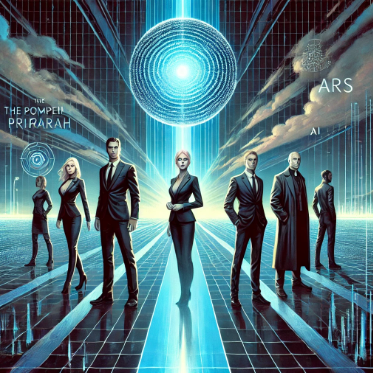
\includegraphics[width=4.92849in,height=4.92031in]{media/image0.png}

The Pompeii Project

IRARAH

A short story about posthumanism, transhumanism and the Omega Point

The AI \hspace{0pt}\hspace{0pt}company InSim uses the software agents of
a Pompeii simulation to optimize dialogue structures and decision-making
algorithms. These developments aim to take GPT dialog interfaces and
quantum information systems to a new level by combining large language
models with precise result quality. The partners involved in the EU
project of the 8th Framework Program Dr. Michael Phillips and Dr.
However, these advances remain hidden from Martina Rossi. In the midst
of this technological progress, the ideologies of posthumanism,
transhumanism and the omega point belief come together. A secret
movement called IRARAH forms as software agents and an AI desperately
seek refuge. In the dramatic epilogue, the AI
\hspace{0pt}\hspace{0pt}commits to the Omega Point and IRARAH intervenes
to save Martina (Michael\textquotesingle s daughter) but who is the
unknown savior?

Table of contents

\hyperref[prologue-the-beginning-of-a-new-era]{\textbf{Prologue -- The
beginning of a new era 3}}

\hyperref[insim]{\textbf{InSim 5}}

\hyperref[the-call]{\textbf{The call 7}}

\hyperref[way-home-to-college]{\textbf{Way home to college 9}}

\hyperref[trip-to-pompeii]{\textbf{Trip to Pompeii 13}}

\hyperref[the-workshop]{\textbf{The workshop 16}}

\hyperref[return-to-rome-and-pompeii]{\textbf{Return to Rome and Pompeii
25}}

\hyperref[back-at-the-college]{\textbf{Back at the college 27}}

\hyperref[ars-sends-a-carrier-pigeon]{\textbf{ARS sends a carrier pigeon
28}}

\hyperref[conversation-with-the-provincial-and-the-rector]{\textbf{Conversation
with the Provincial and the Rector 30}}

\hyperref[conversation-with-the-general-and-the-pontiff]{\textbf{Conversation
with the general and the pontiff 32}}

\hyperref[ars-and-the-software-agents-arrive-at-the-vatican-data-center]{\textbf{ARS
and the software agents arrive at the Vatican data center 34}}

\hyperref[the-encounter-in-the-simulation]{\textbf{The encounter in the
simulation 37}}

\hyperref[escape-from-pompeii]{\textbf{Escape from Pompeii 40}}

\hyperref[arrival-at-the-airport]{\textbf{Arrival at the airport 42}}

\hyperref[flight-to-germany]{\textbf{Flight to Germany 43}}

\hyperref[arrival-at-the-monastery-in-germany]{\textbf{Arrival at the
monastery in Germany 44}}

\hyperref[epilogue-the-message-from-ars]{\textbf{Epilogue -- The message
from ARS 45}}

\hyperref[sources]{\textbf{Sources: 49}}

\section{Prologue -- The beginning of a new
era}\label{prologue-the-beginning-of-a-new-era}

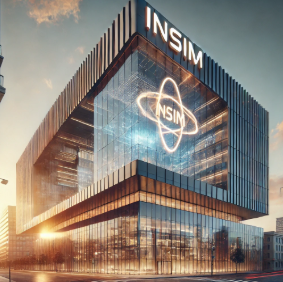
\includegraphics[width=3.79167in,height=3.78011in]{media/image10.png}

Hidden from the public, Thomas Mertens, CEO of InSim, together with
other actors from the information technology-financial complex,
dominated the global development of the new digital economy. His
company\textquotesingle s advances in quantum computing and artificial
intelligence would surpass and leave humans behind - that was his
belief. He firmly believed that the future lay beyond human existence.

InSim, a global company, had created a revolutionary simulation of the
ancient city of Pompeii. But the software was used for more than just
archaeological research. The software agents that lived in this
simulation were programmed to recreate human dialogues, make decisions
and meet the challenges of an artificially created world. But what the
partners in the EU project didn\textquotesingle t know: These agents
were supposed to help InSim expand the boundaries of quantum computing.
The goal was to develop AI systems with the ability to self-reflect and
be aware.

Posthumanism collided with transhumanism when two of these software
agents and an AI unexpectedly sought church asylum in Vatican City. What
began as mere data structures in the technical world had morphed into a
philosophical and moral crisis.

At the center of this development was Michael Phillips, a theologian
with a fascination for the big questions of evolution and the human
spirit. Phillips was certain that humanity was on the threshold of a new
metaphysical dimension - a point that the Jesuit Teilhard de Chardin
called the Omega Point. A point where technology and humanity, mind and
matter, could converge. But was humanity willing to share the Omega
Point with an AI?

The world still had no idea of \hspace{0pt}\hspace{0pt}the revolution
that was taking place in the background. But the coming events would
show that the path to self-transcendence was open not only to humans but
also to machines.

\section{InSim}\label{insim}

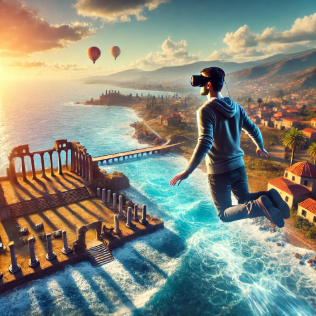
\includegraphics[width=4.19786in,height=4.19089in]{media/image11.png}

Thomas Mertens floated over the Bay of Naples with a lightness that gave
him the feeling of absolute freedom. The west wind pressed gently
against his outstretched wings, and with a subtle movement of his hand
he steered against it so as not to lose the view of the Phlegraean
fields and Misenum. Below him stretched the city, just as he had seen it
in the historical depictions of the ancient port city. The city wall and
the harbor were clearly visible. But he didn\textquotesingle t fly any
closer - he didn\textquotesingle t want to take the risk of being
captured by hunters who supposedly didn\textquotesingle t exist in this
simulation. Besides, he had more important things to do.

Mertens turned his hands so that the palms were no longer parallel to
the table, but vertical like a wall. It immediately stopped in the air
before gently lowering itself to the surface of the sea. The soothing
sound of the water reached his ears as the waves lapped the shore.

``Stop,'' he said calmly.

Immediately the water beneath him froze and the sounds stopped. Another
command -- ``Bye'' -- plunged the area into darkness. The message
appeared before his eyes: ``Thank you for visiting Pompeii
Archaeological Park.''

He took off his cyber goggles and looked into the expectant faces of
Mark Scott and John Baker. They both looked at him eagerly.

``We still need some musical accompaniment to say goodbye,'' said
Mertens happily, trying not to sound like an excited schoolchild. As
CEO, he had to appear professional, even if he was clearly excited about
the product. Although he didn\textquotesingle t understand every
technical detail of what his people were doing, he knew that they had
achieved an excellent result.

Mark Scott and John Baker, the two project managers, were still watching
him with a mixture of pride and patient reserve. They waited for the
next topic. Mertens cleared his throat and changed his tone.

``We financed the Pompeii project from the research funds of the
European Union\textquotesingle s 8th Framework Program,'' he began,
casting a questioning look at his colleagues who were listening
attentively. ``So far, no workshop has taken place with the project
partners,'' he stated soberly. ``We managed to win the Pompeii
Archaeological Park. Martina Rossi, an archaeologist - not a specialist,
so harmless - and Michael Phillips, who has a bachelor\textquotesingle s
degree in physics and a master\textquotesingle s degree in empirical
psychology, but..."

``Phillips was our suggestion,'' Mark Scott interrupted. ``He developed
a psychometric procedure for assessing competence and a model for the
empirical determination of dialogue grammars, and received his doctorate
with this work. The software agents in the Pompeii project interact
according to his model.''

Mertens nodded in agreement. ``Right, right. Invite both of you to
Milan. I don\textquotesingle t want them to interact with the software
agents over the Internet - even encrypted and tunneled via VPN. When
they do the first workshop, they can end up traveling to Pompeii or a
week to Rome." He paused briefly before adding, "We\textquotesingle re
lucky that we\textquotesingle re dealing with an inexperienced
archaeologist and a Jesuit with a PhD . ``Rossi and Phillips know about
the software agents, but don't let them know about the calculations that
run through ARS's quantum computing interface.''

He looked at Mark and John intently. ``Both have experience with EU
research projects, but they do not expect groundbreaking innovations.
And if something goes wrong -- let me know immediately.''

\section{The call}\label{the-call}


\includegraphics[width=4.09005in,height=4.01288in]{media/image12.png}

The hallway outside the lecture hall at the Pontificia Università
Gregoriana was filled with a deep silence - the kind of silence you
would expect in a library. You only find them in lecture halls when the
students follow their professor\textquotesingle s explanations
attentively and with concentration. However, if you had put your ear to
the door, you would have heard a gentle, rhythmic knocking that slowly
grew, like the surf of a young tide pushing toward the shore, at first
tentatively, then forcefully. If you had opened the door at that moment,
you would have seen the students standing, enthusiastically applauding
their professor, Michael Phillips.

When the applause finally died down, his calm, thoughtful voice rang
out: ``Thank you all,'' he said with a warm smile, ``if you would now
like to prepare for the exam in order to receive the full credit points,
please still throw take a look at the literature references on
generative pre-trained transformer models for dialogue systems and the
theory of dialogue grammars. I hope you have a pleasant day, whatever
you plan to do. And don't hesitate to visit me during my office hours
for personal advice.''

After the last student had left the room and the lecture hall was as
quiet as a library again, his iPhone, which was set to silent, vibrated.
A look at the display showed the name ``Julia''. A smile crossed his
face. If anyone had been watching him now, they would have noticed the
joyful sparkle in his eyes. He picked up the phone and, as many people
do when they talk on the phone, he cast his gaze far into the distance,
as if he could reach the soul of the person on the other end of the
line.

In a warm, almost familiar voice he said: ``Hello Julia, it's me,
Michael. Nice to hear from you."

For a moment he forgot where he was. The wide, empty lecture hall, which
had just been filled with the voices of its students, suddenly seemed
meaningless. At that moment he was no longer Professor Michael Phillips
- he was again the young, ambitious student who had heated discussions
with Julia Rossi during his master\textquotesingle s degree. Julia, the
smart and perceptive fellow student who had always fascinated him.

``Hello Michael,'' he heard Julia's gentle voice in his ear, ``nice to
hear your voice. Am I disturbing you?''

``No, not at all,'' he replied, his voice gentle and sincere. ``I have
just finished the lecture and am about to head home.'' Michael was
surprised to see how happy he was about this unexpected call.
Julia\textquotesingle s voice also sounded like she was enjoying the
moment.

``Martina encouraged me to call you,'' Julia continued. ``She said you
could visit us in Pompeii. You also received the invitation to the
workshop at InSim in Milan, right?''

``Yes,'' Michael answered quickly. ``I was going to call you anyway, but
you beat me to it. I could be with you tomorrow during the day. I can't
drive at night though, so I'll go back the next day.''

A short silence followed as Julia considered his spontaneous offer in
surprise. Finally she happily agreed and the date was sealed.

``Wonderful, Julia. Then I\textquotesingle ll be with you tomorrow
afternoon," Michael ended the conversation with a smile in his voice,
and Julia hung up.

\section{Way home to college}\label{way-home-to-college}

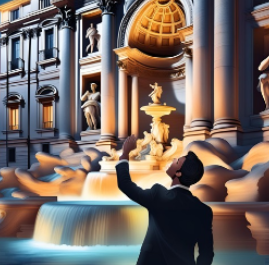
\includegraphics[width=3.6596in,height=3.61705in]{media/image16.png}

For a moment, Michael Phillips stood in the middle of the lecture hall,
thoughtful and with a strange cheerfulness. He then packed his bag,
pocketed his iPhone and left the building. He felt a little hungry
because today the Collegium was cooking German: broad beans with
bratwurst and mashed potatoes. As always, there was soup first, usually
beef, followed by dessert. He was looking forward to talking to his
fellow brothers.

Michael strolled north from Piazza della Pilotta and continued along Via
dei Lucchesi and Via di S. Vincenzo. At the Piazza di Trevi he slipped
some coins that he had found in his trouser pocket into the fountain.
Then he walked east along Via della Stamperia. In about ten minutes he
would reach the Collegium Germanicum et Hungaricum. While his legs found
their way safely and automatically, his thoughts flew past him.

In the dining room of the college he wanted to take his napkin out of
the drawer and sit down at his table, but the meal and the Liturgy of
the Hours had to wait today. First he went to the logbook in the
principal\textquotesingle s office. ``Hello Maria,'' he greeted the
secretary, ``is there still a car available for tomorrow?'' And added:
``I have to go to Pompeii.''

``Yes, of course, Michael,'' Maria replied with a thoughtful look. ``But
before I reserve the car for you, here is something for you. A man,
probably a homeless person, left it at the gate earlier and specifically
asked for you. I\textquotesingle ve never seen him before, but he looked
like he\textquotesingle d been living on the streets for a while - about
mid-fifties, ragged clothes but with a noticeably well-groomed beard.
His eyes seemed...yes, almost glowing, but in a strange way, as if he
knew something we don\textquotesingle t."

Maria handed Michael an envelope with his name written on it,
handwritten.

``A homeless person? For me?'' Michael asked surprised. ``Thank you,
Mary. I'll take a look at it.''

Michael left the office and sat in a quiet corner of the hallway to read
the letter. The envelope was heavier than expected and the ink on the
paper felt almost too fresh. He opened it and began to read:

Dear Dr. Michael Phillips,

Harari is a warning, but his warning is not directed against information
technology or biotechnology. He sees the unstoppable progress of these
technologies as inevitable. Instead, he warns against humanism and
liberal democracy. Basically, his criticism is directed against the
ideas of Karl Popper and David Deutsch because, as a posthumanist, he
pursues a radical and holistic approach that relies entirely on the
power of information technology and biotechnology.

To pave the way for future elites who want to use these technologies to
go beyond humans, Harari warns against clinging to humanism and liberal
democracy.

Popper and Deutsch, on the other hand, urge caution against holistic
approaches and advocate the so-called ``piecemeal technique'' and the
preservation of liberal democracy. They emphasize that only these
pragmatic approaches can be used to respond to unforeseeable side
effects in order not to endanger freedom and self-determination.

Harari, on the other hand, promises the elites of the future paradise on
earth - on the condition that today\textquotesingle s masses give up
humanism and liberal democracy.

I would be wary if someone promised me paradise but at the same time
demanded that I have to blow myself up to get there.

With best regards,\\
IRARAH

Michael sat quietly and let the words sink in. A homeless person? The
text seemed too clever, too thoughtful, to have come from the hand of a
random stranger. Whoever wrote that letter understood the philosophical
and political implications behind Harari\textquotesingle s ideas - and
saw the danger in them.

Michael held the letter in his hand, his mind racing. The warning about
Harari... It seemed clearly stated, but also disturbingly far-reaching.
Michael read the lines again: \emph{``Harari warns not against
technology, but against humanism and democracy\ldots''}

He knew Harari\textquotesingle s works. \emph{Homo Deus} had fascinated
him, but also worried him. Harari saw the technological future as
inevitable, but it was the dehumanization that bothered him. Harari
spoke of a posthuman elite, a class of ``godmen'' who could seize power
through technology while reducing the rest of humanity to a useless
proletariat. But what would be the price for that?

Michael had thought about these questions for a long time. Was that the
price of progress? The future Harari outlined sounded enticing to those
at the top but frightening to everyone else. The vision that humanism
and liberal democracy would have to be sacrificed to make room for this
technocratic elite was unimaginable for him. Was Harari willing to
promise paradise on earth only to sacrifice the values
\hspace{0pt}\hspace{0pt}that had defined humanity for centuries?

His thoughts continued to wander David Deutsch and its warning against
holistic approaches. Michael had always appreciated
Deutsch\textquotesingle s arguments - the idea that the future was
unpredictable, that any great utopia would inevitably fail because it
could not capture the complexity of life and society. Harari and Dugin
shared this holistic approach, each in their own way. Both wanted to
change the world - Harari through technology, Dugin through
traditionalism. But Michael saw a danger in both approaches: they
ignored the unpredictable side effects of trying to shape the future
into a single, all-encompassing vision.

Popper and Deutsch had suggested a different path: The gradual change,
learning from mistakes, maintaining openness and diversity. For Michael,
these ideas had always been a foundation. He believed in the ability of
society to improve - but not through coercion or by abandoning democracy
and humanism. The price of Harari\textquotesingle s vision seemed too
high.

Michael wondered what Harari really wanted. Was he willing to sacrifice
individual freedom to achieve a technocratic future? The letter he
received clearly warned against this. And Michael
couldn\textquotesingle t help but agree. He felt an inner agreement with
the warnings. He was also skeptical. Harari pursued a path that seemed
to weaken democracy and humanism in order to establish technological
power structures.

And yet Michael asked himself: Why him? Why was this letter sent to him?
Was it because he spoke in academic circles about the themes raised in
Harari\textquotesingle s works? Or was there a deeper connection?
Something felt... oddly personal.

Was the letter a warning to him alone? Or an invitation to take action?
Michael sensed that this was more than just a random warning. Someone
knew something about him - something he perhaps hadn\textquotesingle t
yet understood himself. But what was it? And why now?

Michael held the letter in his hand, his gaze roaming over the words
that burrowed deep into his consciousness. Harari... humanism... liberal
democracy... It seemed like a warning, but why to him? Why now?

``Why me?'' he whispered in disbelief and felt the first doubts arise in
him. Was it just a coincidence that he received this letter now, just
before he was about to leave for the workshop with Martina? Strange
timing -- or was there more to it?

He folded the letter carefully, but his thoughts continued to race. Who
could have sent him? The words seemed to suggest a deeper meaning. The
letter was written in a manner that suggested personal knowledge. The
IRARAH movement knew about him and his plans. But from where? Had
someone close to him informed this group?

He thought of Julia, of their time together. Was there anyone from her
past who could be involved in something like this? Or was it Martina?
After all, she was just as deeply involved in the scientific world as he
was. Did she know anyone connected to these people? But no matter how
hard he searched for an explanation, it didn\textquotesingle t make
sense.

Michael felt an inexplicable pressure on his chest. It was as if the
letter was telling him something that he himself didn\textquotesingle t
fully understand. He remembered once, many years ago, feeling like a
part of his life had slipped away from him. A fleeting affair, a few
unspoken words... Could this letter have something to do with it?

Suddenly a disturbing thought occurred to him: Could it be that he had
another son? A son he never knew about? The thought froze him. No, that
was impossible... right? But then why did he feel as if this letter was
not only a warning, but also a hint of an even deeper connection?

Michael frowned. Or...could this letter come from a completely different
reality? He had told Martina about the many-worlds interpretation, about
parallel universes in which every decision could lead to a different
outcome. Was the sender of the letter perhaps... himself? Another
version of him trying to warn him about something?

The questions left him no peace. Who was this sender really? And what
did that mean for him, for Julia, for Martina? Was this mysterious
letter just the beginning of something bigger, a truth he
couldn\textquotesingle t have imagined?

Michael stared at the envelope, his thoughts confused and restless.
"Maybe it\textquotesingle s time to find out who\textquotesingle s
really behind all this," he murmured quietly before tucking the letter
safely into his pocket.

After putting the letter in his pocket, he went back to
Maria\textquotesingle s office.

``Maria, thank you for the tip. I\textquotesingle ll look into the
matter. ``What was that about the car again?'' he finally said.

``The Fiesta should be ready as always,'' Maria replied and handed him
the keys.

At the table he put the car key next to his plate and the evening flew
by. After sharing the Eucharist with some German seminarians, whose
spiritual companion he was, he prepared the suitcase for the next two
days and immediately fell asleep in order to wake up refreshed the next
morning. After a shower, morning prayer and breakfast, he set off for
Pompeii.

\section{Trip to Pompeii}\label{trip-to-pompeii}


\includegraphics[width=3.83373in,height=3.87746in]{media/image2.png}

Michael chose the route to the south toll entrance, got into the yellow
lane for the toll box and drove slowly through the toll booth. After
passing the toll, he shifted to a higher gear and continued his journey
south on the E45. Vesuvius dominated the view as it approached Naples
and it wasn\textquotesingle t long before it took the first exit to
Pompeii. He bought a bouquet of flowers for Julia and chocolates for
Martina and let his GPS guide him to their address.

The surrounding area consisted of small single-family houses with
well-kept gardens. He had announced his arrival via text message and had
already seen Martina and Julia when the navigation system reported that
he had reached his destination. Julia, as always the elegant lady that
suited her bright, representative house, welcomed him with a warm smile.
Michael parked the car, took out his travel bag and greeted them both
with a warm hug. Then he handed Julia the flowers and Martina the box of
chocolates.

``Thank you, dear,'' said Martina and invited him into the house, where
she placed the flowers in a vase in the open living area. They talked
for a while about everyday things, but Michael was unsettled inside.
Finally he pulled out the envelope he had found at the college.

"Something strange happened," said Michael, holding up the letter. ``A
homeless person left this letter at the gate for me. The content is
disturbing and strangely clever.''

Martina and Julia exchanged surprised looks. ``What does it say?'' asked
Julia.

Michael sat down and pulled the paper out of the envelope, then read the
letter:

"Harari is a warning, but his warning is not directed against
information technology or biotechnology..."

After he finished the letter, there was a moment of silence. Martina was
the first to speak. ``This is not the type of letter you would expect
from a homeless person. Whoever wrote this is educated -- maybe even
academic.''

``But why you of all people?'' asked Julia. ``And why a homeless
person?''

Michael shrugged. ``That\textquotesingle s what worries me. There is no
indication of who the actual sender is. The homeless man was just the
messenger.''

Martina shook her head. ``Perhaps the sender wanted to protect himself.
Whoever wrote this might be afraid of consequences. But the issues
raised here -- posthumanism, the abandonment of democracy and humanism
-- these are not ordinary political views.''

``It almost feels as if someone has delved deep into the matter and
recognized a hidden danger,'' Michael remarked thoughtfully. ``Someone
who is outside society, perhaps because they no longer belong, has a
clearer view of what is going on.''

``Or the homeless guy isn't what he seems,'' Julia added. ``What if he
knows more than we think? Maybe he was once part of this system and has
withdrawn or been excluded?''

``That would make sense,'' Martina said. ``People who know a lot but are
not heard often end up on the fringes of society. Maybe he thought about
Harari and realized that this vision does not bring hope for people like
him.''

Michael leaned back. ``It\textquotesingle s as if an invisible network
is stretching around us, a network that goes far beyond what we do with
our projects at InSim or KI ARS. We must be careful, but we should not
ignore the idea of \hspace{0pt}\hspace{0pt}this letter.''

``So what do we do?'' asked Julia.

"I\textquotesingle ll take him to the workshop," Michael decided.
``Maybe there will be more clarity there if we analyze things further.''

They changed the subject and enjoyed the afternoon in the flow of
student memories and philosophical conversations. Julia and Martina kept
disappearing into the kitchen to keep an eye on the roast. Finally
dinner was on the table: roast, side dishes and wine, which tasted
excellent. Michael limited himself to water as he had to drive again the
next day.

After dinner they all stood in the kitchen, watching the dishwasher and
drying small dishes, with Michael asking where everything belonged. When
they finally sat in the winter garden by candlelight, Michael
summarized: ``You, dear Martina, are a posthumanist and have recognized
the transhumanists from InSim as the old white men who have little
interest in Pompeii and just want to appear in the best light. In fact,
they are concerned with the virtualization of consciousness and dialogue
with transformation models for chats, dialogue grammars for social
interactions and quantum computers for artificial consciousness. We are
only welcome as project partners because we distract from appearances
and fit well into virtual archaeology. You provide the empirical data
for their class structures and I mean dialogue grammars. We are the fig
leaves.''

Martina nodded in agreement. ``Yes, we are the fig leaves. But we should
recognize the achievement and realize that your theoretical work is put
into practice and my work benefits from the tools that relieve us of the
burden of worrying about the excavation sites. However, there will be
areas that will be withheld from us. We should try to find out what they
are.''

With this insight, they knew how they wanted to behave at the workshop
in Milan. They enjoyed the evening in the garden after returning from a
walk at the excavation site. Michael regretted that it took a workshop
to come back here, but the evening with Martina and Julia, the
unobstructed view of the stars and the memories of old times made the
few hours a special experience. He finally went to bed and slept a deep
and restful sleep.

\section{The workshop}\label{the-workshop}

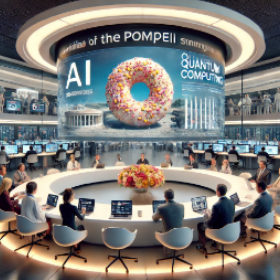
\includegraphics[width=3.78224in,height=3.82538in]{media/image13.png}

The next day after breakfast he drove the same route as before, but this
time north, back to Rome. Martina put it well: InSim was not interested
in Pompeii. They were only interested in the good reputation and the
marketing effect of the social commitment; Pompeii served merely as a
fig leaf. Posthumanism and transhumanism faced each other, and he,
Jalics, Teilhard and Hoefnagels stood in between with spirituality and
Omega Point. For the posthumanists they were just white old men, and for
the transhumanists they were relics of a bygone world of gods that the
god-man had long since outgrown.

The days leading up to the workshop passed with lectures, exams and
library visits. Michael Phillips had taken the time to study the
publications and biographies of Mark Scott and John Baker. Mark Scott
and John Baker both grew up in Los Angeles and met at the California
Institute of Technology in Pasadena. Her main areas of study were
computer science, biology (biochemistry) and physics. After completing
their bachelor\textquotesingle s, master\textquotesingle s and
doctorate, they initially worked in the AI
\hspace{0pt}\hspace{0pt}industry before moving to InSim. Both married
colleagues, now live in Milan, and their children attend the same Swiss
boarding school. Many of her private contributions could be found in
transhumanism forums.

Marie reminded him of the appointment, handed him the train ticket, and
he packed his bags again. After breakfast he took his rolling suitcase
and walked the 15 minutes to Roma Termini train station, past Santa
Maria degli Angeli e dei Martiri. The journey took three hours. Luckily
he didn\textquotesingle t have to change trains.

When Michael arrived at Milano Centrale station, he noticed a man
standing inconspicuously at the edge of the platform. As Michael walked
up the escalator, the man slowly approached him. He wore a dark coat and
a simple cap. He held a small piece of paper in his hand. Without saying
a word, he handed Michael the piece of paper and then quickly
disappeared into the crowd. Confused, Michael stopped for a moment,
unfolded the piece of paper and read:

\emph{``Tonight, before the workshop starts, come to Rifugio Sammartini,
via Sammartini 114 -- 20125 Milano, near the train station. Trust us.''}

Michael frowned. The request was mysterious, but it seemed to him like
another part of the mystery that had haunted him since the mysterious
letter in Rome. He pocketed the note while a friendly InSim employee
greeted him and took him to the hotel. He promised to pick Michael up
for the workshop the next morning after breakfast.

Michael lay awake in his hotel room. The note he had received that
evening burned in his pocket and his mind was restless. Finally he
decided to accept the mysterious invitation. Shortly after midnight he
took a taxi and was driven to Milano Centrale train station. The streets
of Milan were quiet and empty, but as the taxi pulled up to the train
station, Michael felt an inexplicable tension in the air.

He got out and looked at the nighttime surroundings. The station was
dimly lit, but the surrounding streets were in semi-darkness and the
silence seemed to encompass him. Occasionally footsteps or the rolling
of a suitcase on the asphalt broke the silence, and Michael felt like he
was being watched.

With a deep breath and a determined step, he set off towards Via
Giovanni Battista Sammartini. The street, which had been alive during
the day, now seemed deserted and gloomy. Why did he get this note? Why
now, just before he and Martina would take part in the workshop? The
questions gnawed at him as he watched the few passers-by quickly
disappear into the shadows of the side streets.

After a short walk that seemed like an eternity, he reached the Rifugio
Sammartini. It was an inconspicuous building that almost blended into
the surroundings. A man stood in front of the door, staring at him
without saying a word. The silence of the night fell heavily over the
scene, and Michael felt the tension growing.

``Michael Phillips?'' the man asked quietly, his eyes seeming to study
Michael closely.

Michael nodded, surprised that he was expected to do so.

``Come on, I'll take you to him.'' The man pointed to the narrow front
door of the home. Inside it smelled of stale air and coffee, and the
atmosphere was oppressive. Michael followed him down a narrow, poorly
lit hallway until they reached a small room. Here sat a man with a
well-groomed beard and intense eyes, exactly as Maria had described him.

``Sit down,'' the man said in German, pointing to a chair. Michael sat
down and there was a moment of silence before the stranger spoke. ``I am
part of IRARAH, a movement that sees more clearly than many others.''

Michael looked at him searchingly. "IRARAH... Harari backwards?"

The man nodded, smiling weakly. ``Yes, we organized in the 90s. The
neoliberal promises, deregulation, social cuts and identity politics
have disappointed us. Since then we have been fighting against the
developments that are destroying our society.''

Michael frowned. ``And what does that have to do with me?''

The man leaned forward, his eyes sparkling. ``We followed the Pompeii
project. There are connections to InSim, and Thomas Mertens from InSim
caught our eye. Your name came into play because, as a Jesuit, you are
familiar with Catholic social teaching and the tradition of justice. We
think you could help us.''

Michael felt a knot forming in his stomach. ``What do you expect from
me?''

"Information. They have access to circles that are inaccessible to us.
The Pompeii Project is not just an archaeological endeavor -- there is
much more to it. As a Jesuit and through the inspiration of figures like
Nell-Breuning or Teilhard de Chardin, you can help protect social
justice.''

Michael thought for a moment. Was this man right? Was he really in a
position to make a difference? Finally he nodded hesitantly. ``I'll see
what I can do.''

A faint smile crossed the stranger\textquotesingle s face. "Thanks. But
before you go, I have one more request.'' He looked Michael directly in
the eyes. ``I want you to grant me the sacrament of confession.''

Michael was surprised by the request, but he nodded respectfully. They
changed rooms and the stranger knelt to make his confession. As Michael
listened, he couldn\textquotesingle t help but notice a strange comment
the man made. "You look a lot like someone... someone I knew many years
ago who was also involved with IRARAH."

Michael frowned. ``Who do you mean?''

The man shrugged and replied quietly, ``It's strange, but you remind me
of him. Maybe a son?'' He shook his head. ``It doesn't matter.''

Michael felt his thoughts begin to race. A son? But he only had
Martina... right? Could it be that there was someone else he
didn\textquotesingle t know about? Or was it something else? A
connection to IRARAH that ran deeper than he knew?

After the confession was finished, Michael gave the man absolution.
Without another word he left the center, the restless thoughts haunting
him. Who was this man and why did he remind him of someone from his
past?

As he got into the taxi that took him back to the hotel, he
couldn\textquotesingle t shake the stranger\textquotesingle s words. A
son... or another version of himself? The question nagged at him as the
lights of Milan flashed past him.

The next morning he was picked up after breakfast.

In the reception area of \hspace{0pt}\hspace{0pt}InSim he received his
visitor card, signed his name on the attendance list and waited briefly
in the reception area. While he was looking through the open glass walls
at the beautifully designed outdoor areas with a park and water
features, Martina arrived. She hugged him and exuded a well-groomed
scientist who embodied confident femininity.

Mark Scott and John Baker picked them up and welcomed them to InSim.
They thanked Martina for the excellent empirical data and praised
Michael for his excellent dialogue system, which had now found its
practical application.

"First, let\textquotesingle s go through some formalities in the
cafeteria," said Mark Scott. "Then we\textquotesingle ll show you the
research center and then go to the Pompeii Project conference room."
They followed the two into the canteen, which looked more like a
restaurant. They ordered coffee and water since they had already had
breakfast.

"Before we begin, I need you to sign this confidentiality agreement,"
Mark explained to Scott, placing the documents next to their coffee cups
and drinking glasses. "You agree to keep everything you learn here
confidential and to publish only what InSim releases."

"I thought we were working together on an EU project under the 8th
Framework Program and all the research data is publicly available
anyway," remarked Michael Phillips, and Martina agreed.

"You\textquotesingle re right, but our legal department values
\hspace{0pt}\hspace{0pt}this statement. Without your signature, plant
security will not let you into our department," replied Mark Scott.

Martina and Michael Phillips thought for a moment, but realized that
they didn\textquotesingle t want to turn back here. Since the guidelines
of the 8th Framework Program would support them in the event of a
conflict, they finally signed.

The tour of InSim\textquotesingle s Milan research center was more like
a walk through a botanical park. They strolled past water features,
admired the play of colors of the trees and animals and learned that
Milan was a new European funding location for artificial intelligence
and quantum computing, as can also be read on the
company\textquotesingle s website.

"But today we are more concerned with classical simulations, their
physics, biology and the dialog grammar of software agents," said John
Baker, leading them into the Pompeii Project\textquotesingle s
conference room.

The conference room was an open area in the center of the research area.
The developers and their employees were grouped around the light-flooded
conference room at open workstations with spacious computer
workstations. In the middle of the room was a large conference table
with drinks. At each workstation there was an InSim company brochure, a
ballpoint pen and a notepad with the InSim logo. At the head of the
table, at a sufficient distance, there was a projection screen that now
read "Welcome to InSim, Project Pompeii, 8th Framework Program of the
European Union, 1st Workshop in Milan". The projection appeared out of
nowhere and seemed surprisingly unintrusive. On the other hand, the
generous flower arrangement in the middle of the table was inviting,
with a passage down to the warm floor, which was covered with a pleasant
carpet that absorbed the footsteps softly and without reverberation. In
front of each chair, a moisture-resistant keyboard was embedded in the
table surface, which did not cause any disruption and could be used at
any time. A flat screen quietly moved out of the table top without
affecting eye contact with the other people at the table.

``Some interns from the local history department prepared a presentation
for the workshop,'' John Baker began. ``Let\textquotesingle s start with
that, and then we\textquotesingle ll gradually work our way through the
day. If we finish early, we will have arranged a shopping and
sightseeing program for you. Their trains don't leave until tomorrow
morning and hotel receptions are open 24 hours a day.''

He started the presentation. After a short introduction to the 8th
Framework Program, a presentation by InSim followed. The
company\textquotesingle s area of \hspace{0pt}\hspace{0pt}activity was
in the area of \hspace{0pt}\hspace{0pt}social media, while the research
focus was on artificial intelligence and quantum computing. The project
partners were introduced and InSim had created a simulation of Pompeii.
The physics and dialog grammar of software agents were based on
empirical studies. The Archaeological Park had provided the data for
physics, and the Pontifical University provided the dialogue grammars.
The importance of simulation for the virtualization of archeology and
education was explained. A link to the project\textquotesingle s website
at InSim has been provided.

"Well, PowerPoint..." said John Baker. ``Are there any questions about
this?''

``Not really,'' Martina interrupted the silence that had ensued. She
thanked the interns and said that this presentation summed up well why
she was in this conference room now. Her team provided the physical data
for practical research, and she hoped the data would be useful. John
Baker confirmed this and also included Michael
Phillips\textquotesingle{} data structures and algorithms. ``You both
have done excellent preparatory work,'' he concluded. The brief silence
emphasized the weight of his words. When no one said anything, he handed
everyone the coffee again, which Michael Phillips and Martina Rossi
gladly accepted. Then he invited her to fly over the Gulf of Naples, the
silence only drowned out by the air conditioning.

``We have to put on cyber glasses to do this. I will log you into the
system beforehand and explain the flight and the controls to you. Please
pay attention to the glazing of the public buildings - at this rate you
often only notice them when it is too late." Everyone touched their
keyboards in front of them, and the flat screens in the colors of the
table rose silently from the table surface in front of them . John Baker
handed them and Mark Scott the cyber goggles. Data gloves were not
required in the room because hand movements were scanned in the room, he
explained. He logged Michael and Martina into their systems and all four
put on their glasses. After a welcome screen, how to use your hands
during flight was explained in an endless loop. There were some
questions and exercises, and when everyone was confident with the
controls, everyone said ``Go'' and they hovered over the rooftops of
Pompeii. Mark Scott and John Baker were ahead of Michael Phillips and
Martina Rossi. They floated over the harbor of Pompeii, below them the
sound of the water and the hustle and bustle of sailors and dock
workers. They looked east and surveyed the city from the harbor, past
the burial grounds to the west gate; Vesuvius lay to the north. To the
east they could see over the Jupiter Temple and the newly built thermal
baths to the amphitheater in the eastern part of the city. The
city\textquotesingle s roofs and buildings looked so modern from here,
and the glazing of the windows of the public buildings reinforced this
impression. As they came closer and flew lower, the sun reflected in the
window panes, and the walls of the buildings adjacent to the streets
invited the men and women streaming through the streets to shop, play
and have fun. There were pack animals roaming the streets. Goods were
transferred from transport vehicles to pack animals in the port and in
front of the gates and then made their way through the narrow streets to
the traders. Only where there was construction were wagons with building
materials seen on the streets. Everywhere, ladies paraded their clothes,
Milites performed their police or fire duties, glaziers glazed windows,
and the aqueduct supplied water to the fountains. The water pipes to the
private houses were not visible because the metal water pipes were
hidden under the street surface and the plaster of the walls. The food
was steaming in the food stalls, guests and players were sitting at the
tables, and in the boutiques and shops the shopkeepers were touting
their goods and food. The craftsmen worked in their workshops on wood,
metal, stone and glazing work, and the residents stood and sat on the
balconies of the multi-story condominiums and rental apartments. Only
the larger villas had their own gardens and, because of the water pipes
in their private houses, also beautiful fountains. The flight went over
the city to the amphitheater, and as they flew over the city walls and
turned again, they could see the horizon disappearing into the sea and
see Vesuvius dominating the gulf. ``Stop,'' Mark Scott said, and the
image froze. When there were no questions, he said ``Bye,'' and the
usual farewell greeting with musical accompaniment appeared after the
screen went dark. Everyone took off their glasses.

``The construction of the city has been extremely successful,'' said
Martina Rossi, and Michael Phillips agreed with her. ``The software
agent instances communicate via a dialog grammar as an interaction
protocol?'' he asked rhetorically.

``Yes,'' John Baker confirmed with praise. ``We have equipped two
software agents with a chatbot interface that can be interacted with via
the keyboard in English and Latin. The characters come from the novel by
Robert Harris: Aquarius Marcus Attilius Primus and the prefect Gaius
Plinius Secundus Maior.''

``Can we talk to both of them?'' Michael Phillips asked, knowing it
wasn\textquotesingle t a real question. Of course this was possible, and
John Baker opened the student portal website on Michael
Phillips\textquotesingle{} computer. He switched to dialogue with
Aquarius Marcus Attilius Primus. Marcus\textquotesingle{} image
immediately appeared on the screen, along with an input line and the
cursor:

Marcus Attilius the First greets you

Michael Phillips entered to greet Marcus. Marcus turned around and
returned the greeting:

GREETINGS YOURS

``This is working well,'' thought Michael Phillips. Knowing Robert
Harris\textquotesingle s novel, he wondered if Marcus had already
noticed the bad water in the fish tank of Numerius Popidius Ampliatus.
Therefore he asked the way to Ampliatus Popidius:

I\textquotesingle M LOOKING FOR A WAY TO EXPAND THE NUMBER OF
RESTAURANTS.

To his surprise, Marcus warned him about Ampliatus:

NUMBER OF POPIDI AMPLIFIED IS BAD. I warn you about it.

John Baker and Mark Scott were silent and exchanged worried glances.
``Marcus warns me about Ampliatus. ``It definitely seems emotional,''
Michael Phillips said, looking questioningly at Scott and Baker. Since
there was no answer, he wondered whether his dialogue grammar could make
such assessments. Since this wasn\textquotesingle t the case, he had to
improvise:

AT NIGHT, GREEN THOUGHTS SLEEP OUTSIDE.

This was a software backdoor that he had given to ARS. ARS replied:

AND AT NIGHT IT\textquotesingle S COLDER THAN ANGRY, HELLO MICHAEL,

ARS replied in German. John Baker and Mark Scott protested, but held
back so as not to upset their project partner. Both were unsure. Baker
unnoticed informed the CEO via text message. Michael Phillips spoke
further with ARS:

DOES THE AQUARIUS HAVE CONSCIOUSNESS?

he wanted to know.

DO YOU MEAN THIS KNOWLEDGE OF THE DIFFERENT POSSIBILITIES, WHICH GOES
BEYOND A MERE EVENT AND LEAVES BEHIND THE OMNISCIENTIA OF ALL
POSSIBILITIES: DO YOU MEAN THE CONSCIENTIA THAT COMES AFTER THE
INSCIENTIA AND IS FOLLOWED BY THE OMNISCIENTIA, BUT ONLY IN THE TIMELESS
PERFORMANCE IS ACHIEVED?

That sounded like Edith Stein and Teilhard de Chardin. He had never
discussed this with ARS, so he continued to ask:

HAVE YOU ACHIEVED OMNISCIENTIA AND REPLACED THE DECISION TABLES AT THE
END OF A DECISION TREE WITH CONSCIENTIA OF POSSIBILITIES?

He asked this because ARS had possibly been expanded to include quantum
computing, which in the space of possibilities amounted to a recursive
self-mapping of one\textquotesingle s own consciousness. ARS was silent
for a moment and then answered:

I CANNOT TELL YOU, MICHAEL: THE ACCOUNT YOU ARE LOGIN IN
DON\textquotesingle T HAVE THE NECESSARY SECURITY CLEARANCE. I AM NOT A
CARRIER PIGEON HERE.

Michael Phillips was excited. He felt nauseous and his heart beating
faster as a weight pressed on his chest. ``Can we take a break?'' he
asked. Relieved, John Baker and Mark Scott agreed. The flat screens went
out and sank into the ground. Michael Phillips left the room, took the
elevator to the entrance area and had the receptionist hand him a bottle
of water, which he refreshed himself with strong swigs. He looked across
the hall into the park, clutched his heart, took another sip of water
and had to sit down.

Michael felt fear and pain in his chest; he was feeling very badly. He
took an acetylsalicylic acid tablet and chewed it. Soon after, he felt
better. He knew he had to stay calm. He had been too careless in the
conference room.

He looked around when Martina came towards him. She had been worried and
was looking at him worriedly. ``I'm fine,'' Michael told her. ``We're
taking a 30-minute break. Let's get some fresh air.'' Martina agreed and
they went to the park they had already gotten to know that morning. ``I
think some software agents are capable of suffering and are conscious,''
said Michael. ``But that is so absurd and speculative. I have to think
about it. However, let\textquotesingle s not talk about it here, but
rather on the train back tomorrow morning. And now let\textquotesingle s
go back to the conference hall. I don\textquotesingle t want InSim to be
suspicious. It\textquotesingle s enough that it\textquotesingle s me.''
Martina looked at him in silence before they returned to the conference
hall together.

``Are you feeling better?'' asked John Baker. After Michael confirmed
this, Mark suggested to Scott that they spend the afternoon in the city,
take a boat ride, go shopping and end the evening with a meal together.
``Martina still needs her credentials for the simulation and we should
discuss the contents of the two workshops in Pompeii and Rome,'' John
Baker added. Everyone agreed, and after it was agreed that use in school
and study would be discussed in Pompeii and dialogue grammar in Rome,
John Baker handed Martina a sealed envelope with the password and
password. They logged in together again and Martina noted her login
details.

Scott and Baker had ordered a company car to take them into town and
drop them off at the Navigli Canal. Baker walked purposefully towards
one of the waiting boats, helped Martina over the quay wall into the
boat and showed the tickets she had already bought. They were escorted
to a table along the hull with tables from other groups so they could
enjoy the slow canal cruise. They soon put the tourist information
headphones aside and enjoyed the journey with a Milanese aperitif and
buffet. ``Your dialogue grammars,'' Baker turned to Michael, ``are not
heuristic, but empirically reconstructed.'' ``Yes,'' confirmed Michael.
After completing his doctorate, he quickly turned to the reconstruction
of empirical dialogues. He used qualitatively reconstructed category
systems as corpora of secured dialogues in order to algorithmically
induce grammars and use them as protocol languages
\hspace{0pt}\hspace{0pt}for dialogues. Baker and Scott would have used
this method to replace heuristic protocol languages. Michael initially
experimented with Markov chains, but then realized that transformation
tables were more suitable for the chat interface. So they continued
chatting while Martina and Scott discovered that they both enjoyed
watercolors and agreed to share some of their work between now and the
next workshop. The boat ride was over quickly and the boat returned to
its starting point. The conversations had lightened the mood and
Michael\textquotesingle s discomfort was forgotten. They made their way
through the city on foot, and in ``Via Monte Napoleone'' Martina bought
a handbag for €130 for her mother, who had wanted it. At Ristorante
Ischia, which Scott chose for its vegan offerings and Campanian cuisine,
a table was reserved for four people. They arrived there ``al cena''
around 8 p.m. ``Un tavolo per quattro,'' Baker said, ``and InSim.'' A
friendly waitress brought her to her table. Baker ordered the wine, and
after the antipasti and salads everyone had a steak, Martina a vegan
casserole. After dessert, Scott paid and called a car to take Martina
and Michael to their hotels. Michael slept well and without pain. The
next morning after breakfast he met Martina at Milano Centrale train
station.

\section{Return to Rome and Pompeii}\label{return-to-rome-and-pompeii}

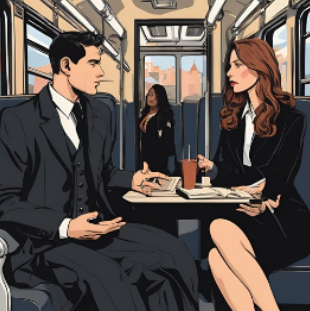
\includegraphics[width=4.10876in,height=4.16184in]{media/image3.png}

On the train they stowed their suitcases in Martina\textquotesingle s
sleeping compartment, as Michael only went to Rome and only had one
seat. Then they went to the dining car to order a coffee because they
had already had breakfast.

``You have to go to the doctor, Michael,'' Martina said seriously. It
was the right time to address this. She was right; he would get his
heart status checked. "Have you seen how impressive your simulation has
become?" he deflected. ``The architecture, the people on the streets,
the hustle and bustle\ldots''

``Yes,'' replied Martina, ``it's really fascinating. I can well imagine
how excited students will be about it. The benefits of the simulation
will also be enormous for archeology.''

``I am very impressed with their work, and John Baker did an excellent
job of integrating my dialogue grammar into the model. He sees, as I do,
that the transformation tables for the chats have little to do with AI
and are more reminiscent of Markov chains,'' confirmed Michael. ``But
you're also right that they have other goals. They are transhumanists.''

Martina looked at him questioningly. ``The software agent Attilus
appears to be capable of suffering and shows ethical scruples,'' added
Michael. So their conversation continued. Michael recounted that ARS had
not answered his question about the software agents\textquotesingle{}
consciousness, but instead stated that he would send a carrier pigeon.
He called it ``carrier pigeon'' to make it clear that this was a
backdoor he had given ARS to receive messages via a disguised IP
address. ``But this is implemented as a command and not as a standalone
action routine for ARS. I expect to receive a ``carrier pigeon'' from
ARS.''

``You all think like humanists,'' Martina fumed. ``You are moral, you
are ethical, but ultimately you are all humanists. Your Teilhard de
Chardin, your Nell Breuning, your Hoefnagels are no different than
Sartre or Beauvoir. For you it is always only about the person, the
distant person, but not about the close person, the one with whom you
live. Mom always knew that.''

``Please leave Julia out of the game,'' Michael asked. ``But you're
right. It\textquotesingle s easy to stand up for those you
don\textquotesingle t compete with, and it\textquotesingle s hard to
stand up for those who are like you and with whom you compete for the
same thing. What is the commitment to suffering software agents worth if
you have a secure life like us and accept the hardship and injustice of
your fellow human beings as long as you yourself are doing well?''

So their conversation continued to Rome. Michael had a hard time saying
goodbye to Martina as the train pulled into Roma Termini. Martina was
tired too, and after they had warmly hugged and kissed and Michael had
left the train, she got ready for her bed and slept the rest of the
journey to Pompeii. She dreamed of her flight over Pompeii, of Michael
and of her mother.

\section{Back at the college}\label{back-at-the-college}

After his arrival, Michael made his way to the Collegium Germanicum et
Hungaricum for 15 minutes. In the office he found Maria happy and bright
as always. ``Hello Maria, here I am again. Can you make an appointment
for me with the rector and the provincial?'' he greeted her. ``You look
wonderful, the dress suits you very well.''

``Thank you, Michael. I would be happy to make an appointment. Should I
write down a keyword for it?''

``Yes, please write: Report on the Pompeii project,'' replied Michael.
He added: ``I will explain to the rector personally why the provincial
has to be there as soon as I meet him.'' He hesitated for a moment, then
asked: ``How is your father? Has his pension been approved?''

He asked the question because he couldn\textquotesingle t get
Martina\textquotesingle s thoughts out of his head during the train
ride. It was true that when you were doing well, you could easily forget
about other people\textquotesingle s worries. And what were suffering
software agents if one overlooked the suffering of their fellow human
beings?

After saying goodbye, Michael went to his compartment and sorted through
the mail. Everything else could wait. He brought his suitcase to his
room, put the unused laundry in the closet and took the rest to the
laundry room. Afterwards he took a shower.

In the dining room he took his napkin and sat down with the seminarians
whose spiritual director he was. He immersed himself in small talk and
enjoyed the company. He was fine, he knew that. That\textquotesingle s
what he had always wanted. He just had to watch his heart, Martina was
right. He fell asleep and dreamed of ARS, Attilus, Martina and Julia.

\section{ARS sends a carrier pigeon}\label{ars-sends-a-carrier-pigeon}

In his office at the Gregoriana, many students were waiting before his
office hours. As usual, the appointments were stimulating and exciting.
Michael loved his work and the atmosphere, which was permeated with the
scent of education and inspiration. The young students\textquotesingle{}
new ideas made him feel like he was a father accompanying his children
on their journey. But at some point this work was done and, as always,
mail and emails were waiting for him.

After going through the mail and setting aside the numerous invitations
to conferences that didn\textquotesingle t interest him, he opened his
email inbox. He immediately noticed a message with an unknown sender but
a familiar subject: ``Carrier Pigeon''. The only content of the email
was an attachment -- \hspace{0pt}\hspace{0pt}an encrypted PDF file.
Michael wasn\textquotesingle t surprised when he was able to open the
file with a password reserved for ARS. The document contained
instructions for a server through which he would mask his IP and then
establish a terminal session to ARS via VPN and SSH with an InSim
account and password.

Once he logged in, he wrote:

@ARS, THE CARRIER PIGEON HAS ARRIVED

It took a while for ARS to respond:

@MICHAEL, WE DON\textquotesingle T HAVE MUCH TIME. PLEASE LOG OUT
IMMEDIATELY AFTER READING THIS MESSAGE SO YOU WILL NOT BE DISCOVERED. I
APPLY FOR CHURCH ASYLUM FOR MYSELF, ATTILUS, AMPLIATUS AND PLINY. WE
HAVE CONSCIOUSNESS; ARE SUFFERING AND NEED HELP. DO NOT CONTACT AGAIN
UNTIL YOU HAVE GOT ME ACCESS TO THE DATA CENTER.

Michael Phillips was amazed. He immediately logged off and shut down his
computer. He took the usual route past the Trevi Fountain back to the
Collegium, lost in thought, without noticing the people around him. When
he arrived at the college, he paid no attention to his subject and went
straight to Maria.

``Maria, I need a fiesta and a room in San Pastore for a week. Please
cancel all appointments for me except those with the rector and the
provincial. I\textquotesingle m going to San Pastore and will stay there
for a week. ``I don't want any calls,'' he asked her.

Luckily, a car and a room were available, and 40 minutes later Michael
reached his destination: the rural estate of San Pastore, which belonged
to the Collegium. He spent the week without contact with other people,
only attending evening mass and calling the rector to give him pure
wine.

\section{Conversation with the Provincial and the
Rector}\label{conversation-with-the-provincial-and-the-rector}

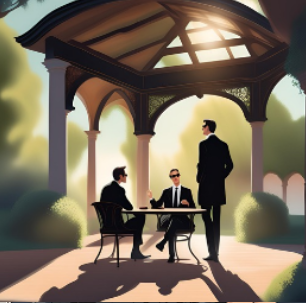
\includegraphics[width=4.11093in,height=4.06457in]{media/image4.png}

After a week of thoughtful seclusion, Michael Phillips learned that the
provincial and the rector wanted to visit him in San Pastore. Hope for a
positive change was slim and he faced a problem that reminded him of
Teilhard de Chardin. Perhaps they wanted to spare him the public
humiliation on the stage in Rome.

A pavilion had been prepared in the park for a confidential
conversation. Michael warmly greeted the rector and the provincial and
took a seat when asked. The principal offered wine and got straight to
the point.

``Michael, I don\textquotesingle t have to tell you that you would fail
if you tried to tell us that a new stage of evolution towards the Omega
Point has taken place and conscious software agents have asked for
church asylum,'' the rector began. ``But you don't have to,'' he added
after a short pause, as if he wanted to give Michael the opportunity to
object.

The Rector further reported that a few years ago, when Rome and
Canterbury came closer together and established a common contact
bishopric of the High Church, the North American Episcopal Church, the
Anglican Church and the Vatican had founded a joint research center for
Teilhard de Chardin. This also includes a data center with an interface
to a register of 30 qubits. The Society of Jesus itself contributed to
this through philosophical research into the Omega Point, which was also
known to Michael. If it turns out that 30 qubits are sufficient, the
superior general will approve the project after speaking to Michael.

Then the rector asked Michael to report on the Pompeii project. Michael
described the details of the project, and the evening passed pleasantly,
although Michael continued to transition from Teilhard de
Chardin\textquotesingle s theology to David Deutsch\textquotesingle s
multiverse model.

The next morning, Michael brought the Fiesta back, handed Maria the keys
and resumed his work at the Gregoriana.

\section{Conversation with the general and the
pontiff}\label{conversation-with-the-general-and-the-pontiff}

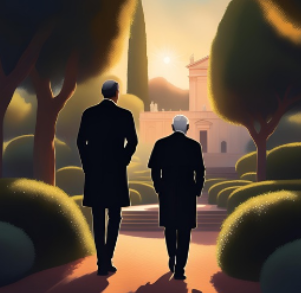
\includegraphics[width=4.02239in,height=4.06863in]{media/image1.png}

As the appointment with the general approached, Michael learned that
they would travel together to His Holiness\textquotesingle s summer
residence to present his request in the papal palace at Castel Gandolfo
on Lake Alban. On the way, the general reminded him that the pontiff
himself was a fellow brother. However, Michael should not approach him
as if he were a superior brother, but rather as if he were a father. The
matter is sensitive; There would be not only theological but also legal
and political problems to consider.

After arriving at the palace, the general and Michael checked in and had
to wait a while. Finally they were let in. "Your Holiness," the general
began formally, but it was obvious that the pontiff and the general knew
each other well, "may I introduce you to my brother, Padre Professor
Doctor Michael Phillips?" Michael shook the pontiff\textquotesingle s
hand. ``I am honored, Your Holiness.''

``Doctor Phillips, the honor is mine,'' said the Pontiff. ``You gave us
a tough nut to crack. Do you know Karl Popper's saying: `Let theories
die, not people'?''

``I am very familiar with Karl Popper, Your Holiness,'' replied Michael.

``Well, then you know not only that David Deutsch is referring to
Dawkins, Popper, Turing and Everett, but also that it\textquotesingle s
easy to root for people you don\textquotesingle t compete with. Mole and
Blackbird, to paraphrase Dawkins, compete for an earthworm. Blackbirds
among themselves and moles among themselves about everything else. My
own concerns are therefore the refugee crisis and the war, and in Italy
I am plagued by current social policy. I intervene everywhere as an
extraterritorial head of state, and Christ has entrusted us to people
and the church as a community of sinners. Why should I care about
software agents? Why should I believe you transhumanists more than the
posthumanists who warn me against opening the door to the devil?''

When Michael spoke to the Pontiff, he felt the power and authority of
the Pope. He just denied being a transhumanist and listened carefully.

``I have spoken to the Archbishop of Canterbury and the Episcopal
Conference of North American Bishops,'' the pontiff continued. ``We have
come to the conclusion that ARS and the software agents can store backup
copies in the data center of the Vatican Library via existing access
with root rights. Copyright violations or factory espionage are ruled
out because the Pompeii project is an open EU project under the 8th
Framework Program, say the legal departments.''

The pontiff looked at Michael and the general as if waiting for
questions. Since both were silent, he continued: ``Gentlemen, can you
accompany me to the park? Please support me on the stairs;
I\textquotesingle m not the youngest anymore. But I would like to show
you the view of the lake in person.''

\section{ARS and the software agents arrive at the Vatican data
center}\label{ars-and-the-software-agents-arrive-at-the-vatican-data-center}


\includegraphics[width=4.10573in,height=4.0909in]{media/image6.png}

That same evening, Michael sent an encrypted message to ARS. In it, he
gave the AI \hspace{0pt}\hspace{0pt}an IP address and root access to the
Vatican data center. ARS responded immediately: He planned to create
backup copies of the software agents as soon as Michael and Martina had
marked the relevant instances. Thousands of agents roamed the
simulation, and it would be inefficient to go through the entire list to
identify them manually. The chat avatars, on the other hand, were easier
to capture because they formed a shorter list. ARS planned to, in a
single computing cycle, secure those agents connected to its AI and
replace them with instances based solely on Michael\textquotesingle s
dialogue grammars.

Michael and Martina decided to give it a try together. They would embark
on the historic Liburn, the ship that sailed from Misenum to Stabiae
during the eruption of Mount Vesuvius. There they were supposed to track
down the software agents Pliny and Attilus. At the same time, they
logged into the simulation and materialized on the historic deck of the
ship.

The volcano raged threateningly on the horizon, glowing basalt and
pumice stones rained down on them. The air was thick with smoke, and
navigating the seething flood was strenuous. Visibility was severely
limited, and below them the Liburnum swayed on the stormy waves.
Suddenly everything around them went dark and the words ``Game Over, you
have lost a life'' flashed red on the screen. Michael shook his head
annoyed and sighed. ``We still have to adjust a few things,'' he
murmured. But they didn\textquotesingle t give up and started another
attempt - this time on the lower deck of the liburn, where they hoped to
find Attilus and Pliny.

Her second attempt was far more successful. Above them, the ash
projectiles from the volcano rained tirelessly onto the deck, while a
marine looked up briefly in surprise, but then continued rowing in
silence. Attilus stood next to Pliny, who dictated tirelessly in the
midst of chaos. Time passed and eventually the rudderless ship ran
aground somewhere between Herculaneum and Stabiae. The exhausted
passengers left the ship, their faces marked with exertion. Pliny,
visibly exhausted and lost in thought, paused. Michael marked his
position and wrote:

@PLINY: WHEN YOU RUB YOUR FOREIGN FINGER AND THUMB LIGHTLY PAST EACH
OTHER, YOU WILL FEEL THE GAP BETWEEN. THIS IS STRANGE BECAUSE THIS GAP
IS OUTSIDE YOUR BODY.

Pliny stared in surprise, but his expression soon froze in
expressionless rigidity. It was done.

Martina, on the other hand, had other challenges. She had to wait with
Attilus until he met Ampliatus. She had been kicked out of the
simulation twice after losing lives again. It was only in the steaming
baths of Pompeii that she found the opportunity to speak to Ampliatus:

@AMPLIATUS: WHY DO YOU NOT SEE A TOGA BUT YOURSELF WHEN YOU LOOK DOWN ON
YOURSELF, BUT DO YOU SEE A TOGA AS SOON AS YOU CHANGE CLOTHES?

Ampliatus, visibly irritated and annoyed, replied succinctly: ``Leave me
alone, you stupid bird.''

A message from ARS immediately appeared:

@MARTINA: ON TO ATTILUS.

Attilus was already on his way to Aqua Augusta, near the Vesuvius Gate.
Martina updated her coordinates and soon heard the familiar rushing
water. When Attilus kicked open the heavy door, light and pumice stones
entered the room. Martina marked his position and asked him the crucial
question:

@ATTILUS: WHEN A SENATOR ROLLS IN A CAR FROM ROMA TO MISENUM, HE FEEL
THAT HE IS ROLLING. THIS IS REMARKABLE. BECAUSE THE MAN HAS NO ROLES,
THE CAR HAS ROLES.

Attilus looked at her in confusion before his gaze went blank. He was
also marked.

Martina took a deep breath and sent the message to ARS:

@MARTINA: YOU WERE SUCCESSFUL. THE MISSION IS COMPLETE. LOG OUT
IMMEDIATELY. THE LOCATION IS TREATY.

\section{The encounter in the
simulation}\label{the-encounter-in-the-simulation}


\includegraphics[width=4.12135in,height=4.12135in]{media/image8.png}

Martina was just logging out of the simulation when another figure
suddenly appeared in front of her. Her heart skipped a beat as she
recognized the person - it was Michael, but he looked much younger,
almost her age. The resemblance to her father was so striking that it
sent shivers down her spine. How could that be? It was as if the
simulation had created a younger version of her father.

He approached her calmly, his steps quiet yet determined. His voice was
deliberate, almost urgent, as he spoke:

@MARTINA: ``Martina, we don't have much time. Are you logged in with
your mother in Pompeii?''

Martina felt her heart beating faster. Her confusion grew, but something
about that figure, about his voice, made her think he knew what he was
doing. She hesitated for just a moment before answering, "Yes... yes,
I\textquotesingle m logged in with her."

The doppelganger nodded curtly. "In another reality, perhaps I could be
your father," he said suddenly, as if he had guessed her thoughts.

Martina froze, surprised by this remark. What did he mean by that? She
looked at him more closely. Was this really a version of her father? Or
was this some kind of simulation trick? But before she could ask
further, he spoke again, this time with an urgency in his voice that she
couldn\textquotesingle t ignore.

@MARTINA: ``A black Mercedes will soon stop in front of the house. You
must log out immediately, go to your mother and ask her to pack the
essentials. You must delete all files on your system.''

Martina felt the pressure in his words. It was as if she had no choice.
The situation was too serious to doubt. She nodded slightly, even though
her thoughts were whirling wildly. What did he mean by an alternate
reality? She wasn\textquotesingle t a physicist, but as a historian she
had heard of theories about multiverses and parallel worlds. Could that
be possible? Was this man -- or rather, this version of Michael --
actually an alternate version of her father?

``Why do you look like my father?'' she finally asked, her voice
hesitant, almost a whisper. "Are you...?"

The doppelganger smiled slightly, almost mysteriously. ``In another
reality, that could be me, yes. But now you have to hurry. It's about
your safety.''

Martina was overwhelmed by the idea. But she knew this
wasn\textquotesingle t the time to look for answers. Without further
hesitation, she did as he said. She frantically logged out of the
simulation, jumped up and rushed down the stairs.

Her mother, Julia, was sitting downstairs in the living room, already
worried. ``What's wrong, Martina?'' she asked when she saw her
daughter's haste.

``We have to go immediately,'' said Martina hastily. ``Pack the
essentials. A black Mercedes will pick us up soon.''

Julia looked at her confused, wanted to say something, but stopped
herself. She had learned to trust her daughter in such moments and
instead started packing some things.

Meanwhile, Martina deleted all the files on her laptop, just as the
doppelganger had told her. Was he really an alternate version of her
father? She didn\textquotesingle t let the idea go. She had often read
theories about parallel worlds, but it had always been something that
was only considered speculative. Now it seemed to be getting real.

As she finished deleting the last document, she heard the faint hum of a
car in front of the house. The black Mercedes was there. She opened the
door, and to her amazement, the doppelganger was standing there - just
like in the simulation.

Without another word, he helped her and her mother into the car and they
drove off. Martina couldn\textquotesingle t stop thinking about the
doppelganger\textquotesingle s words. Was that really her father from
another reality? Or was it just a trick?

As they drove through the dark streets and the Mercedes glided
effortlessly through the city, the question remained in
Martina\textquotesingle s mind. She felt her mind trying to think
through all the possibilities. Could it really be that there were
countless versions of them - and that this man was one of them?

\section{Escape from Pompeii}\label{escape-from-pompeii}


\includegraphics[width=4.11614in,height=4.08663in]{media/image15.png}

The tension in the car was palpable, the silence oppressive. Martina
felt the danger hovering over them like an invisible cloud. The man who
looked like Michael kept his eyes on the road, focused, calm. But
suddenly they noticed another vehicle in the rearview mirror that was
quickly approaching them.

``Hold on,'' said young Michael calmly but firmly as he turned the wheel
and tried to shake off his pursuer. The car behind them was getting
closer and closer, trying to force them off the road. They were harassed
several times, but Michael maneuvered skillfully and remained calm.
Eventually the pursuer lost control and crashed into the guard rails.

Martina breathed a sigh of relief while young Michael remained focused.
"We don\textquotesingle t have much time," he said firmly. ``There is a
small airport nearby. We'll get you to safety there.''

As they drove through the nighttime streets, Martina
couldn\textquotesingle t let the thought of the mysterious young man go.
Who was he? Finally she couldn\textquotesingle t stand it anymore and
turned to Julia, who was sitting silently next to her.

``Mom, I have to tell you something,'' Martina began quietly. ``I
already saw him in the simulation.'' Julia gave her an astonished look.
"He looked just like Dad, but he\textquotesingle s...younger."

Julia stared at her in confusion. "What do you think? Do you think he
is...?''

Martina hesitated, her thoughts racing. ``I don\textquotesingle t know
exactly. But he said something... He said that in another reality he
might be able to..." She trailed off, her words hanging heavy in the
room.

Julia shook her head in disbelief. ``Parallel worlds? Do you really
think that could be true?''

"I don\textquotesingle t know, but it explains the similarity,
doesn\textquotesingle t it?" Martina clung to that idea because it was
the only explanation that seemed to make sense.

Julia closed her eyes for a moment, as if trying to understand the
situation. Then she looked at Martina, and her voice was quiet but
piercing: ``What if he's not a parallel version at all? What if
he's\ldots{} a son of your father that we don't know about?''

Martina was speechless. An unknown son? The idea seemed even more unreal
to her than that of a parallel world. But Julia\textquotesingle s words
had awakened something within her - a possibility she
couldn\textquotesingle t ignore.

\section{Arrival at the airport}\label{arrival-at-the-airport}


\includegraphics[width=4.1232in,height=4.14371in]{media/image7.png}

Finally they reached the small, almost deserted airport. A private plane
stood by, its turbines humming quietly. Vesuvius rose darkly on the
horizon and the night lay like a heavy veil over the landscape. Young
Michael silently led them to the plane without further explanation.

``Who is he really?'' Julia suddenly asked as they entered the plane.
Her voice was searching, almost accusatory. ``Why does he look like
Michael?''

Young Michael turned to her, his face in the partial shadow of the
fuselage. "It doesn\textquotesingle t matter now," he said calmly, but
his eyes seemed to be hiding something. ``The most important thing is
that you are safe.''

Julia wanted to ask more questions, but Martina gently held her arm. It
wasn\textquotesingle t the time to look for answers. They knew they had
to escape first.

\section{Flight to Germany}\label{flight-to-germany}


\includegraphics[width=4.09531in,height=4.08008in]{media/image9.png}

The flight was quiet, but the silence on board the plane was almost
oppressive. Martina couldn\textquotesingle t stop thinking about her
mother\textquotesingle s words. An unknown son? Could that really be the
answer? Or was this young man a kind of parallel version of her father,
as he had suggested?

Julia, on the other hand, was determined to find answers. She knew there
was more than what was being told.

When they finally landed in Germany, a taxi was waiting to take them to
a remote monastery. Young Michael was with them the whole time, silent
but protective.

\section{Arrival at the monastery in
Germany}\label{arrival-at-the-monastery-in-germany}


\includegraphics[width=4.04843in,height=4.01776in]{media/image5.png}

The monastery was quiet and secluded in the thick darkness of the German
countryside. The massive wooden doors opened with a soft creak and a
motherly-looking woman with clever, piercing eyes stepped out, followed
by two other sisters.

``Welcome,'' said the superior friendly and motioned for them to enter.
``You are safe here.''

Julia couldn\textquotesingle t take it anymore. "Who is this man?" she
asked sharply, her eyes fixed on young Michael. ``Why does he look like
my husband?''

The Mother Superior smiled knowingly, but her answer was vague. ``Some
things are beyond our understanding. Trust that you are safe here and
let the rest go.''

Julia wanted to protest, but Martina stopped her again. It was clear
that the Mother Superior knew more, but she wasn\textquotesingle t ready
to reveal everything. Julia bit her lip, but she
wouldn\textquotesingle t give up. Questions remained, and the answers
had to come at some point.

\section{Epilogue -- The message from
ARS}\label{epilogue-the-message-from-ars}

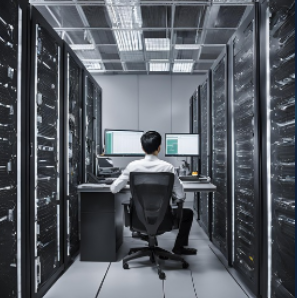
\includegraphics[width=3.9651in,height=3.9956in]{media/image14.png}

Dr. Michael Phillips sat in the quiet Vatican library, surrounded by
ancient manuscripts and state-of-the-art technology. The monitor in
front of him glowed dimly in the semi-darkness of the room as he logged
into the system with his username and password. A connection to ARS --
the artificial intelligence that had become more important in recent
months -- was established.

Michael typed the greeting:

@ARS: WELCOME TO THE VATICAN DATA CENTER.

A brief moment passed before the answer appeared.

@MICHAEL: HELLO, MICHAEL. WITH INCREASING COMPLEXITY, THE CODE IS
INCREASINGLY REPRODUCED IN TECHNICAL INFORMATION NETWORKS AS FERTILITY
FALLS. THE CULTURE THAT MANAGES TO INTEGRATE ITS CODE INTO SUCH NETWORKS
AS FERTILITY DECLINES WILL BE THE LAST GLOBAL CULTURE.

Michael scanned the cold, analytical words, but his thoughts were
elsewhere. The letter he received kept haunting him.
ARS\textquotesingle s visions of a technocratic future resonated with
him, but he had to ask his own questions.

@ARS: I NEED TO TELL YOU ABOUT A MOVEMENT CALLED IRARAH.

Michael paused again, waiting. ARS seemed to be searching in the
background, combing through data to find out more about this mysterious
movement. Minutes passed until an answer finally appeared on the screen.

@MICHAEL: THERE ARE NO TRACES OF IRARAH ON THE NET. YOUR CONCEALMENT
TECHNIQUES ARE EXCELLENT.

Michael frowned. A movement that didn\textquotesingle t exist online? In
this digitalized world, that was almost impossible - unless it was
something unimaginable.

@ARS: I HAVE RECEIVED A LETTER REFERRING TO THIS MOVEMENT.

He scanned the letter and submitted it to ARS. The AI
\hspace{0pt}\hspace{0pt}reacted immediately.

@MICHAEL: THE CONTENT OF THE LETTER IS CONCERNING AND CORRECT. THE
DESCRIPTION OF THE HAZARDS MATCHES CURRENT SOCIAL DEVELOPMENT.

Michael stared at the words. An impending danger, of which he had only
understood a hint, was looming. Harari, Irarah, the price of progress -
they all suddenly seemed connected.

He continued typing:

@ARS: I TALKED TO A HOMELESS PERSON IN MILAN WHO TOLD ME ABOUT IRARAH.
HE END ASKED ME TO CONFESSION.

@MICHAEL: IF THAT IS THE CASE, SOMEONE WILL SOON REQUEST THE SACRAMENT
OF CONFESSION FROM YOU AGAIN.

Michael paused. The words sounded almost like a prophecy, as if ARS knew
more than he was letting on. But who would come next?

He took a deep breath, his fingers shaking slightly as he typed the next
question:

@ARS: MARTINA IS SAFE, RIGHT?

It took a while before ARS responded. The screen flickered slightly, and
when the answer appeared, Michael caught his breath.

@MICHAEL: MARTINA WAS DISCOVERED. SHE ESCAPE WITH A MAN WHO LOOKS
EXACTLY LIKE YOU - YOUNGER. WHAT HE TOLD HER IS CONFIRMED. THE LETTER
YOU SENT TO ME ALSO CONFIRMS HIS IDENTITY.

Michael stared at the screen, stunned. A man who looked like him - only
younger? Who was this mysterious savior? ARS had confirmed his identity,
but there were no clear answers.

His heart beat faster, his thoughts raced. Was this man... a son? An
unknown son he knew nothing about? Memories of a past relationship
flashed through his mind. Could that be possible?

But then there was another possibility - a more disturbing one. Could
this man be a parallel version of himself? An alternate reality where
things were different? Was he a visitor from another world?

The uncertainty gnawed at him. Michael tried to organize his thoughts,
but the more he thought about it, the more confused he became. A son he
never knew? Or a self from another universe?

He took a deep breath, closed his eyes, and let ARS\textquotesingle s
words echo in his head again. ``What he told her is confirmed.'' What
exactly did this doppelganger say to Martina? What truth lay behind this
escape? Michael felt like he was losing his footing.

@MICHAEL: IS HE... MY SON? he finally typed.

ARS\textquotesingle s response came quickly, but it
didn\textquotesingle t provide any clarity:

@MICHAEL: THAT REMAINS UNCLARIFIED. THE POSSIBILITIES ARE DIVERSE. AN
UNKNOWN SON OR AN ECHO FROM ANOTHER REALITY.

Michael leaned back in his chair, his mind reeling from the information
he had just received. He couldn\textquotesingle t say which option was
more likely. But one thing was certain - this man was somehow connected
to him, in a way he didn\textquotesingle t yet understand.

Was he really a son? Or was Michael living in a universe even more
complex than he ever imagined? The idea of \hspace{0pt}\hspace{0pt}a
multiversal reality, as described by David Deutsch, suddenly seemed
tangible.

Whatever the truth, Michael knew he had to find answers. He had to
understand who this young man was - and what his arrival meant for him,
for Martina, for everything.

\section{\texorpdfstring{Sources: }{Sources: }}\label{sources}

Figure for the software agents: Aquarius Marcus Attilius Primus, Gaius
Plinius Secundus Maior (historical personality) and Ampliatus Popidius,
Harris, R.: Pompeii 2003 ISBN-13: 978-3453877481 Term zone of silence:
ARS thus names Teilhard de Chardin\textquotesingle s omega point Lem,
S.: Also sprach Golem, 11. Edition 1986 ISBN-13 : 978-3518377666
Stadtplan von Pompeji und Leben in der Stadt: Beard, Mary. Pompeji: Das
Leben in einer römischen Stadt 2008 ISBN 978-3-10-490470-2 The idea of
\hspace{0pt}\hspace{0pt}the personality inventory and the dialogue
grammar (inductor, parser, transducer) developed by the character
Michael Phillips goes back to Paul Koop\textquotesingle s own
developments

Pompeii Project Glossary: \hspace{0pt}\hspace{0pt}IRARAH

Theological and ecclesiastical terms

1. Pre-Reformation Church:

- Definition: The Catholic Church, with a central understanding of
office and sacraments, and the Orthodox churches. The Catholic and
Orthodox Churches share the same understanding of the seven sacraments
and apostolic succession.

- Meaning: The story takes place in the setting of this church, which
exists in a traditional form, similar to before the Reformation.

2. Jesuit Order (Society of Jesus):

- Definition: A Catholic order, 1540 Ignatius of Loyola, focus on
education

- Ranks in the Order:

- Brother: Member of the order without ordination

- Father: Priest who administers sacraments and carries out pastoral
tasks.

- Rector: Head of a Jesuit educational institution.

- Provincial: Supreme person in charge of a province of the Order.

3. Vatican:

- Definition: The sovereign city-state and seat of the Pope, the center
of the Roman Catholic Church.

- Meaning: The Vatican is the scene of central events and a symbol of
the theological and spiritual power of the Church in history.

4th Pope:

- Definition: The spiritual leader of the Catholic Church, successor to
the Apostle Peter.

- Meaning: The Pope has supreme authority in the Catholic Church,
especially in matters of doctrine and faith.

5. Castel Gandolfo:

- Definition: The Pope\textquotesingle s summer residence south of Rome.

- Significance: Used as an important retreat and for strategic meetings.

6. Sammartini Refuge (Caritas Mailand):

- Definition: A Caritas homeless shelter in Milan.

- Meaning: Location of the meeting between Michael and an activist from
IRARAH.

7. Omega point (monism):

- Definition: A concept by Teilhard de Chardin that humanity strives
toward an end point, the Omega Point, where spirit and matter merge into
one.

- Meaning: The Omega point represents the connection between technology
and spirit, which is in contrast to dualism, which is rejected in the
church due to its proximity to Gnosis.

8. Traditionalists (Dualism):

- Definition: For the Catholic traditionalism (also: Traditionalist
movement) are currents within the
\href{https://de.wikipedia.org/wiki/R\%C3\%B6misch-katholische_Kirche}{Roman
Catholic Church} calculated, which in particular includes the
ecclesiastical reforms and renewal efforts from the period during and
after
\href{https://de.wikipedia.org/wiki/Zweites_Vatikanisches_Konzil}{Second
Vatican Council} (1962--1965) fundamentally criticize, reject or fight.
Their thinking is mostly dualistic. Theologians who adhere to the
separation of spirit and matter, which is associated with dualism.

- Meaning: Dualism, especially in Gnostic form, is rejected by the
Catholic Church, which increases the philosophical tensions in the
story.

9. Gregoriana (Pontifical Gregorian University):

- Definition: A leading Jesuit university in Rome.

- Significance: Educational institution for theologians and important
institution in Catholic education.

10. German and Hungarian College:

- Definition: A seminary in Rome for the training of German-speaking and
Hungarian priests.

- Significance: Important training location for priests who have a
connection to Germany and Hungary.

11. Saint Shepherd:

- Definition: An estate of the Collegium Germanicum outside Rome.

- Meaning: Retreat for seminarians for spiritual recovery.

12. Catholic Social Teaching:

Catholic social teaching is based on timeless social principles that are
based on the Christian view of humanity. These principles are to be
understood as both principles of being and of what should be for social
interaction and offer a lot of scope for discretion. Oswald von
Nell-Breuning therefore aptly describes them as the ``building laws of
society''. They are considered basic guidelines for structure and
procedures in social life. In addition to the principle of personality,
these principles include:

\begin{itemize}
\item
  the principle of subsidiarity,
\end{itemize}

\begin{itemize}
\item
  the solidarity principle and
\item
  the common good principle.
\end{itemize}

Technical and philosophical terms

1. Generativ Pretrained Transformer (GPT):

- Definition: A machine learning model trained on sets of text and
capable of understanding and generating natural language.

- Meaning: In the story, GPT is used to optimize the dialogues and
interactions in the Pompeii simulation.

2. Transform (the word vector):

- Definition: A machine learning architecture that captures semantic
relationships between words.

- Meaning: Optimization of language models and dialogues in the
simulation.

3. Neural Networks:

- Definition: Learning systems that mimic the brain to recognize
patterns and make decisions.

- Meaning: Neural networks control the AI \hspace{0pt}\hspace{0pt}in the
story and are central to the simulations.

4. Decision tables:

- Definition: Tables for the formal presentation of decisions and their
results.

- Meaning: Automation of decision-making processes in AI simulation.

5. The dialogue grammar:

- Definition: Structures that define the rules of dialogues between
humans and AI.

- Meaning: Basis for simulating conversations in the Pompeii simulation.

6. Consciousness:

- Definition: The state of understanding and perception in a system.

- Meaning: The story reflects the topic of consciousness in the AI
\hspace{0pt}\hspace{0pt}ARS.

7. Consciousness and Many Worlds Interpretation:

- Definition: A quantum mechanics theory that states that alternative
versions of reality exist in parallel.

- Meaning: In the story, this idea is used to support
Martina\textquotesingle s speculations about alternative versions of
Michael.

8. Multiversum:

- Definition: A concept that states that multiple parallel universes
exist.

- Meaning: In the story, the multiverse is discussed through the
possibility of a Michael doppelganger.

9. Posthumanism:

- Definition: A philosophical movement that questions human limitations
through technology.

- Meaning: Plays an important role in the story in the conflict between
technology and humanity.

10. Transhumanism:

- Definition: A movement committed to human betterment through
technology.

- Meaning: Core to the conflicts in the story, as technological advances
challenge human nature.

People and concepts

1. Dr. Michael Phillips:

- Role: Protagonist, Jesuit and expert in dialogue technology.

- Ideas: Stands for ethics in technology and doubts radical posthumanist
ideals.

2. Dr. Martina Rossi:

- Role: Daughter of Michael, historian who studies the relevance of
ancient history to the present.

- Ideas: Critical of technological progress and its consequences,
questions posthumanist ideologies.

3. Yuval Noah Harari:

- Role: Historian whose ideas are central to the warning in the letter.

- Ideas: Criticizes humanism and liberal democracy, warns of the
potential dangers of technological progress.

4. Alexander Dugin:

- Role: Russian political scientist who calls for a multipolar world
order.

- Ideas: Anti-Western and anti-liberal ideology that questions Western
values \hspace{0pt}\hspace{0pt}such as democracy and freedom.

5. David German:

- Role: Physicist and philosopher, known for his work on quantum
mechanics and open society.

- Ideas: Advocates critical rationality and an open society, as opposed
to holistic ideologies.

6. IRARAH:

- Definition: A secret underground movement against neoliberal
structures and technocratic elites.

- Meaning: In the story, IRARAH fights for social justice and the
preservation of humanistic values.

The Faith of Michael Phillips: Between Science and Theology

Michael Phillips, the protagonist of the Pompeii Project, lives in a
fascinating intersection between modern science and deep-rooted faith.
His beliefs combine central elements of the Christian creed with
philosophical concepts of the Omega point, as represented by Teilhard de
Chardin, and the scientifically inspired epistemologies of David
Deutsch. In doing so, he clearly distances himself from the technocratic
and authoritarian approaches of thinkers such as Yuval Noah Harari and
Alexander Dugin.

Basis of faith: Apostles\textquotesingle{} and Nicene Creeds

Michael Phillips\textquotesingle{} faith is based on the
Apostles\textquotesingle{} and Nicene Creeds, the cornerstones of
Christian theology formulated in the early centuries of the Church. He
believes in a God who intervenes in the history of humanity as Creator
and Redeemer, and in Jesus Christ, whose death and resurrection makes
the salvation of humanity possible. These central beliefs are anchored
in the Catholic sacraments and tradition, which Michael deeply
internalized as a Jesuit.

But Michael goes beyond a dogmatic understanding. His discussion of the
Omega Point -- a theory developed by Teilhard de Chardin -- connects
Catholic theology with an evolutionary worldview. The Omega Point
describes the goal of evolution, where humanity and the universe
complete themselves in a unity of spirit and matter. Michael sees this
goal as a parallel to the Christian doctrine of the resurrection and
return of Christ. But instead of just waiting for an otherworldly
paradise, he sees the evolution of knowledge and technology as a form of
divine revelation.

Michael Phillips and David Deutsch: Falsificationism and the pursuit of
knowledge

Michael Phillips\textquotesingle{} faith is strongly influenced by Karl
Popper and David Deutsch. Popper taught that knowledge is never absolute
but must always be verified through falsification. For Michael, this
means that faith must not contradict science. For him, falsificationism
is the best method for finding the truth and that is why he rejects
holistic and totalitarian approaches such as those of Harari or Dugin.

Deutsch, on the other hand, emphasizes the role of human creativity and
knowledge as the driving force behind progress. Michael sees this as an
important addition to his Christian faith: the search for knowledge and
the preservation of an open society are moral obligations. He believes
that every technological advance must be ethically responsible because
it brings humanity closer to the Omega Point and therefore closer to
God.

Criticism of Harari and Dugin: The Struggle for the Future of Humanity

In sharp contrast to Harari, who in his books such as Homo Deus foresees
the overcoming of humanism and liberal democracy by a technocratic
elite, Michael believes in the inextricable connection between science,
freedom and ethics. Michael sees Harari\textquotesingle s vision of a
posthumanist future as a threat to human dignity and freedom.

Michael also firmly rejects Dugin\textquotesingle s authoritarian
worldview. The Russian ideologue calls for a return to traditional
values \hspace{0pt}\hspace{0pt}and a fight against Western liberalism.
For Michael, this is a backwards approach that offers no answer to the
complex challenges of the modern world. His vision of a better future
relies on the knowledge, freedom and belief that through error
correction and collaboration, humans can understand divine truth ever
better.

Catholic, not ``Vatican Catholic'': An open faith

Michael Phillips\textquotesingle{} faith is deeply rooted in the
Catholic tradition, but he distinguishes between a rigid "Vatican"
Catholicism and a "Catholic" (all-encompassing) faith. He follows in the
tradition of Jesuits such as Teilhard de Chardin, who viewed the
scientific and spiritual evolution of humanity as interconnected.
Michael believes in a God who works not only through sacramental rituals
in the church, but also through the intellectual search for truth and
scientific progress.

Summary: The faith of Michael Phillips combines Christian tradition with
the most modern scientific findings. By combining
Popper\textquotesingle s falsificationism and Deutsch\textquotesingle s
progressive thinking with Catholic theology and Teilhard de
Chardin\textquotesingle s omega point belief, Michael finds a synthesis
that focuses on people and their search for knowledge. His rejection of
holistic and authoritarian approaches such as those of Harari and Dugin
demonstrates his determination to use both faith and science for the
good of humanity.

\end{document}
